%%%%%%%%%%%%%%%%%%%%%%%%%%%%%%%%%%%%%%%%%
% University/School Laboratory Report
% LaTeX Template
% Version 3.1 (25/3/14)
%
% This template has been downloaded from:
% http://www.LaTeXTemplates.com
%
% Original author:
% Linux and Unix Users Group at Virginia Tech Wiki 
% (https://vtluug.org/wiki/Example_LaTeX_chem_lab_report)
%
% License:
% CC BY-NC-SA 3.0 (http://creativecommons.org/licenses/by-nc-sa/3.0/)
%
%%%%%%%%%%%%%%%%%%%%%%%%%%%%%%%%%%%%%%%%%

%----------------------------------------------------------------------------------------
%	PACKAGES AND DOCUMENT CONFIGURATIONS
%----------------------------------------------------------------------------------------

\documentclass{article}

\usepackage[version=3]{mhchem} % Package for chemical equation typesetting
\usepackage{siunitx} % Provides the \SI{}{} and \si{} command for typesetting SI units
\usepackage{graphicx} % Required for the inclusion of images
\usepackage{natbib} % Required to change bibliography style to APA
\usepackage{amsmath} % Required for some math elements
\usepackage{mathrsfs} 
\usepackage{enumerate} % Required for the enumerate function
\usepackage[siunitx]{circuitikz} % Required for the drawing of circuit diagrams
\usepackage{caption}
\usepackage{graphicx}
\usepackage{subcaption}
\usepackage{xfrac}
\usepackage{float}
\usepackage{enumitem}
\usepackage{chemgreek}
\usepackage{pgfplots}
\usepackage[margin=0.5in]{geometry}
\usepackage{epstopdf}

\setlength\parindent{0pt} % Removes all indentation from paragraphs

\renewcommand{\labelenumi}{\alph{enumi}.} % Make numbering in the enumerate environment by letter rather than number (e.g. section 6)

%\usepackage{times} % Uncomment to use the Times New Roman font

%----------------------------------------------------------------------------------------
%	DOCUMENT INFORMATION
%----------------------------------------------------------------------------------------

\title{Instrumentation \\ Computer Simulation Assignment \\ ENG342} % Title

\author{Shane \textsc{Reynolds}} % Author name

\date{\today} % Date for the report

\begin{document}

\maketitle % Insert the title, author and date

\begin{center}
\begin{tabular}{l r}
Date Performed: & August 13, 2017 \\ % Date the experiment was performed
Instructor: & Dr Suresh Thennadil % Instructor/supervisor
\end{tabular}
\end{center}

% If you wish to include an abstract, uncomment the lines below
% \begin{abstract}
% Abstract text
% \end{abstract}

%----------------------------------------------------------------------------------------
%	SECTION 1
%----------------------------------------------------------------------------------------

\section{Objective}

An ideal tank heating process scenario will be mathematically modelled. Comparison the model will compared to simulated results, and discussed.

%----------------------------------------------------------------------------------------
%	SECTION 2
%----------------------------------------------------------------------------------------

\section{Background \& Model Derivation}
Consider the tank shown in Figure 1. Assuming that there is no heat transfer through the walls of the tank the \textbf{LAW OF WHAT} suggests that:
\begin{align}
\Bigg[\parbox{3cm}{Rate of heat from incoming liquid}\Bigg] - \Bigg[\parbox{3cm}{Rate of heat form outgoing liquid}\Bigg] + \Bigg[\parbox{3cm}{Rate of heat into tank from heater}\Bigg] = \Bigg[\parbox{3cm}{Rate of heat accumulation in tank}\Bigg]
\end{align}

Heat energy for a given liquid is given by \textbf{LAW OF WHAT}:
\begin{align}
Q = m \cdot C_p \cdot (T - T_{ref}),
\end{align}
where $Q$ is ????, $m$ is mass, $C_p$ is specific heat capacity, $T$ is temperature, and $T_{ref}$ is a reference temperature. Rates of heat into the tank due the feed can be found from derivative of (1) with respect to time.
\begin{align}
q_{in} = \frac{dm_{in}}{dt} \cdot C_p \cdot (T_i - T_{ref}),
\end{align}
where $T_i$ is the input temperature from the feed.

Similarly, we find the rate of heat out of the tank from the output as:
\begin{align}
q_{out} = \frac{dm_{out}}{dt} \cdot C_p \cdot (T - T_{ref})
\end{align}

The accumulation of heat in the tank, $Q_T$, is given by the following relationship:
\begin{align*}
Q_{T} = M \cdot C_P \cdot (T - T_{ref})
\end{align*}

Differentiating this expression, we get the rate of heat change in the tank accumulation is given by:
\begin{align}
q_{T} = M \cdot C_P \cdot \frac{dT}{dt} = \rho \cdot V \cdot C_P \cdot \frac{dT}{dt}
\end{align}

Substituting equations (2), (3), and (4) into equation (1), we get the following expression:
\begin{align*}
\frac{dm_{in}}{dt} \cdot C_p \cdot (T_i - T_{ref}) - \frac{dm_{out}}{dt} \cdot C_p \cdot (T - T_{ref}) + q_h = \rho \cdot V \cdot C_P \cdot \frac{dT}{dt}
\end{align*}

Noting that $\omega = \frac{dm_{in}}{dt} = \frac{dm_{out}}{dt}$, we can write:
\begin{align}
\omega \cdot C_p \cdot (T_i - T_{ref}) - \omega \cdot C_p \cdot (T - T_{ref}) + q_h = \rho \cdot V \cdot C_P \cdot \frac{dT}{dt}
\end{align}

Considering, this equation in the steady state, yields:
\begin{align}
\omega \cdot C_p \cdot (T_{is} - T_{ref}) - \omega \cdot C_p \cdot (T_s - T_{ref}) + q_h = 0
\end{align}

Subtracting equation (7) from equation (6) yields
%----------------------------------------------------------------------------------------
%	SECTION 3
%----------------------------------------------------------------------------------------

\section{Time Response of Open Loop System}
Section 2 defined the theoretical model of the system as:
\begin{align*}
T'(s) = \bigg(\frac{1}{\tau s + 1}\bigg) \cdot T'_i(s) + \bigg(\frac{R}{\tau s + 1}\bigg) \cdot q_h(s)
\end{align*}

In order to specify the model fully, the time constant, $\tau$, and the resistance, $R$, need to be calculated. If the tank capacity, $V$, is 1000$\si{\liter}$, the fluid density, $\rho$, is 1$\si{\kilogram\per\liter}$, and the volumetric flow rate, $v_f$, is 200$\si{\liter\per\minute}$.\\

The time constant, $\tau$, is determined as:
\begin{align}
\tau = \frac{\rho \cdot V}{\omega} = \frac{\rho \cdot V}{\rho \cdot \omega} = \frac{1000}{200} = 5\si{\minute}
\end{align}

The resistance is determined as:
\begin{align}
R = \frac{1}{\omega \cdot C_P} = \frac{1}{\rho \cdot v_f \cdot C_P} = \frac{1}{836.8}\si{\minute\degreeCelsius\per\kilo\joule}
\end{align}
\subsection{Time Response for Step Increase in Feed Temperature, With Heat Input Held Constant}
Holding the heat input to the system constant, a step increase in the feed temperature was input to the system. The mathematical model in the Laplace domain can be seen in equation (XX):
\begin{align}
T'(s) = \frac{1}{5 \cdot \tau + 1} \cdot T'_i(s)
\end{align} 

Given a deviation in the input temperature, $T'_i(t)$ , of 10$\si{\degreeCelsius}$, we note that the Laplace transform is:
\begin{align*}
\mathscr{L}\{T'_i(t)\} &= \mathscr{L}\{10 \cdot u(t)\}\\
T'_i(s) &= \frac{10}{s}
\end{align*}

The mathematical model, in the Laplace domain, becomes:
\begin{align}
T'(s) = \frac{10}{s \cdot (5 \cdot s + 1)}
\end{align}

Solving this system yields the following expression for the temperature deviation in the time domain:
\begin{align}
T'(t) = 10 \cdot (1 - e^{-\sfrac{t}{5}})
\end{align}

The plot of this model can be seen in Figure XX. A simulation of the system was run in Simulink using the block diagram shown in Figure XX. The step input, and simulated system response can be seen in Figure XX.

\begin{figure}[h]
\centering
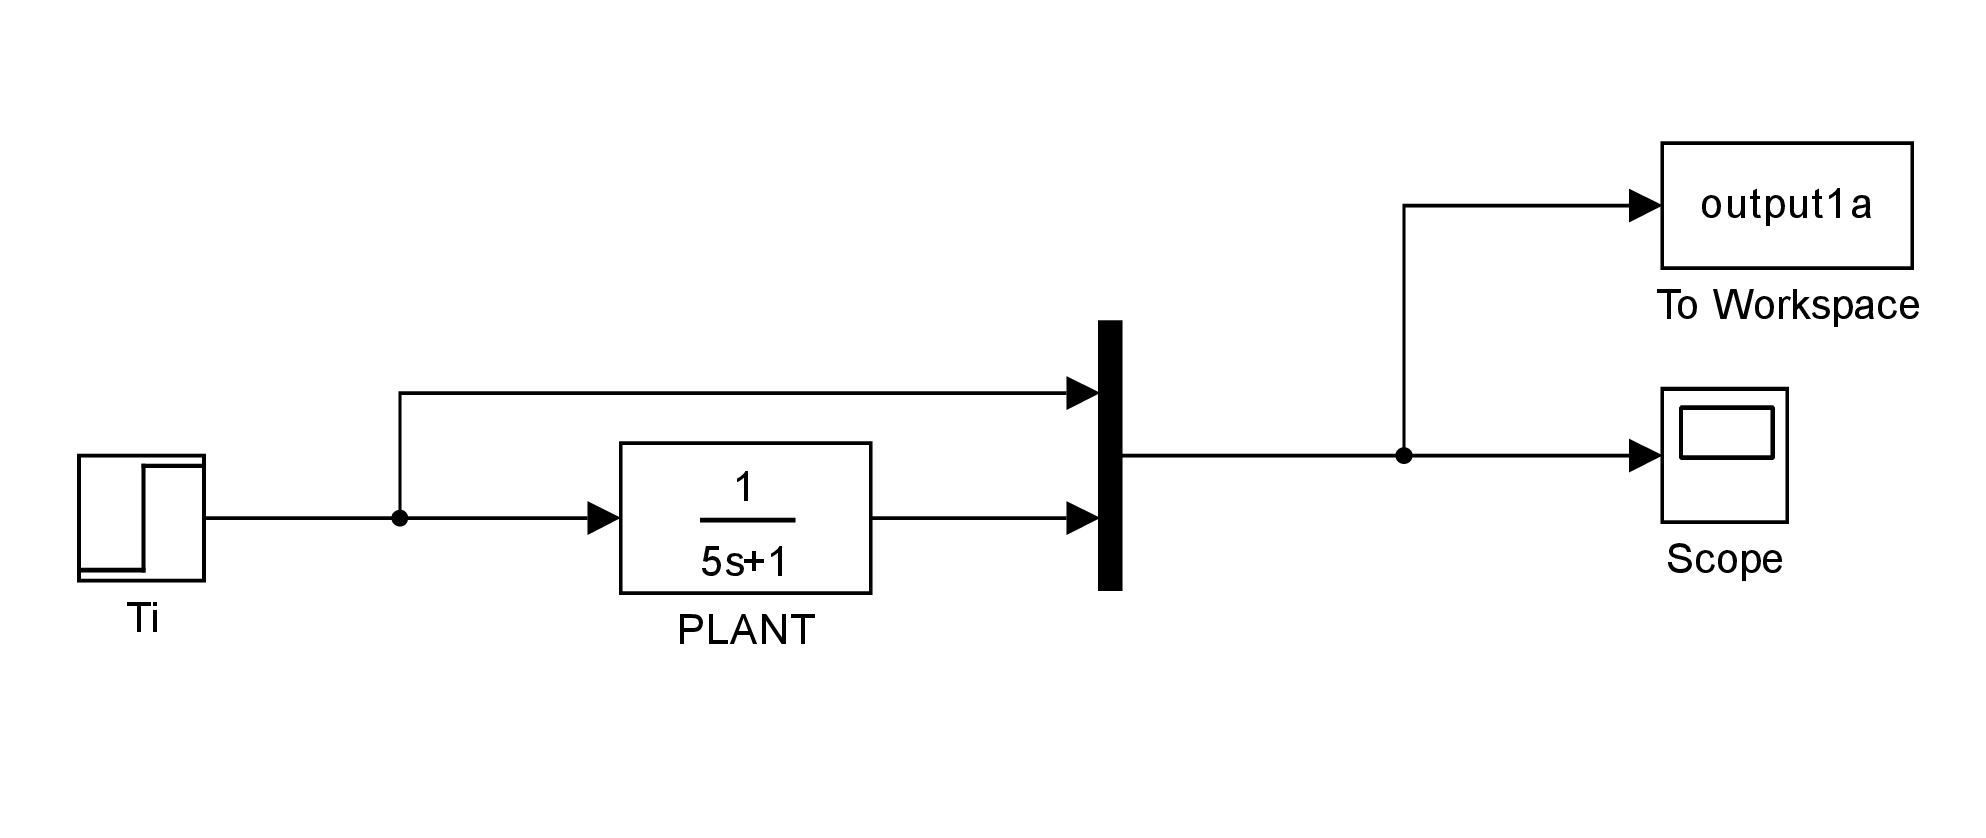
\includegraphics[scale=0.2]{block_1a}
\caption{text}
\end{figure}

\begin{figure}[h]
\begin{minipage}{0.45\textwidth}
\centering
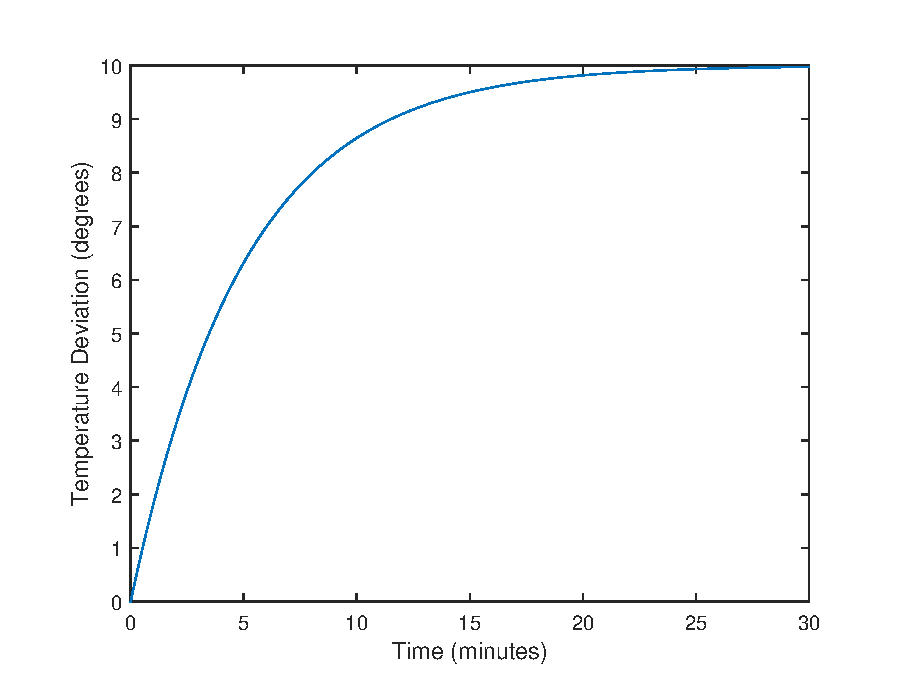
\includegraphics[height=6cm]{1a_mod}
\caption{Temperature deviation model, shown in equation (12), for a step change in the feed temperature of 10$\si{\degreeCelsius}$, holding the heat input constant}
\end{minipage}
\hspace{1cm}
\begin{minipage}{0.45\textwidth}
\centering
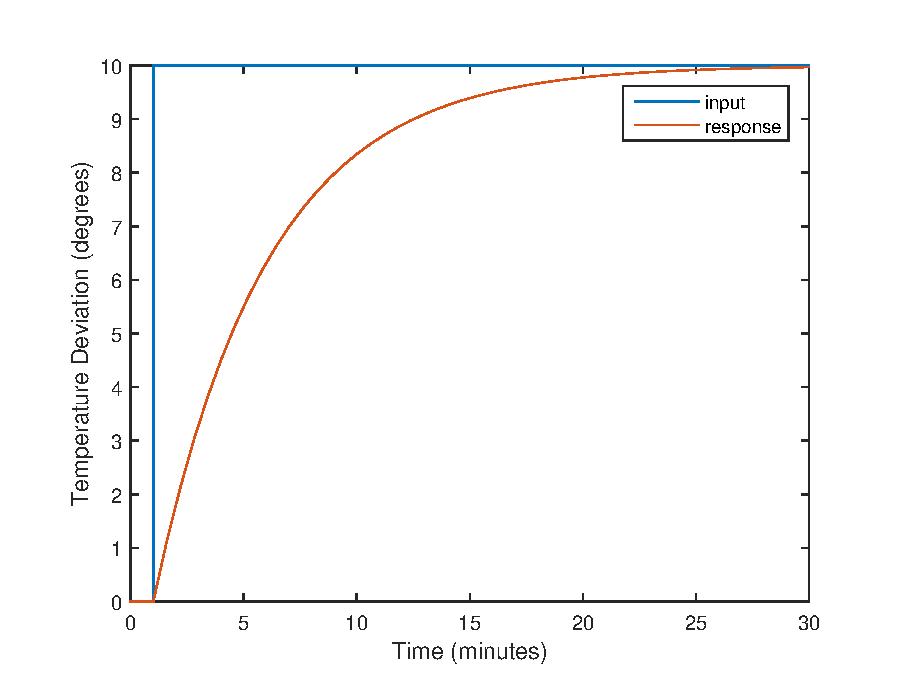
\includegraphics[height=6cm]{1a_sim}
\caption{Temperature deviation simulation for a step change in the feed temperature of 10$\si{\degreeCelsius}$, holding the heat input constant}
\end{minipage}
\end{figure}

\subsection{Time Response for Step Increase in Heat Input, With Feed Temperature Held Constant}
Holding the feed temperature to the system constant, a step increase in the heat input introduced to the system. The mathematical model in the Laplace domain can be seen in equation (XX):
\begin{align}
T'(s) = \frac{1}{5 \cdot \tau + 1} \cdot T'_i(s) + \frac{\sfrac{1}{836.8}}{5 \cdot \tau + 1} \cdot q'_h(s)
\end{align} 

Given a deviation in the heat input, $q'_h(t)$ , of 42$\si{\kilo\watt} = 2520\si{\kilo\joule\per\minute}$ and an increase in the feed temperature of 10$\si{\degreeCelsius}$, we note that model shown in equation XX can be re-written as:
\begin{align}
T'(s) = \frac{2520}{s \cdot (5 \cdot s + 1)}
\end{align}

The mathematical model, in the Laplace domain, becomes:
\begin{align}
T'(s) = \frac{2520}{s \cdot (5 \cdot s + 1)}
\end{align}

Solving this system yields the following expression for the temperature deviation in the time domain:
\begin{align}
T'(t) = 3 \cdot (1 - e^{-\sfrac{t}{5}})
\end{align}

The plot of this model can be seen in Figure XX. A simulation of the system was run in Simulink using the block diagram shown in Figure XX. The step input, and simulated system response can be seen in Figure XX.

\begin{figure}[h]
\centering
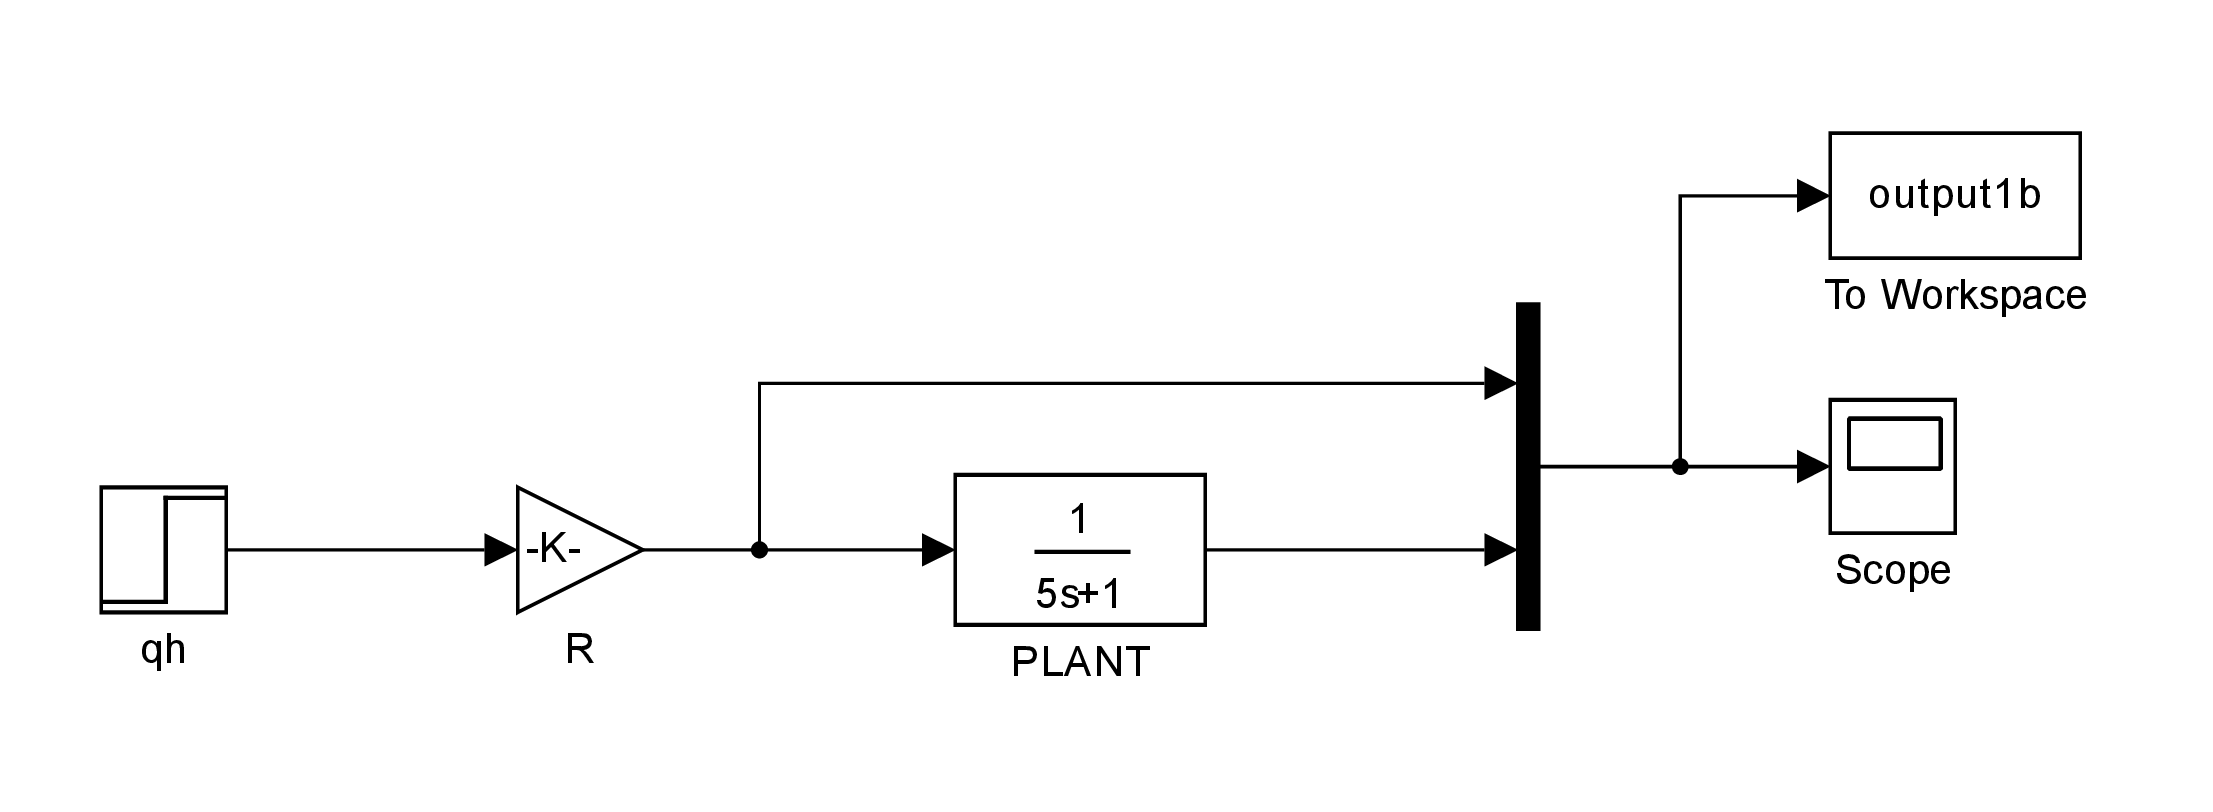
\includegraphics[scale=0.2]{block_1b}
\caption{text}
\end{figure}

\begin{figure}[h]
\begin{minipage}{0.45\textwidth}
\centering
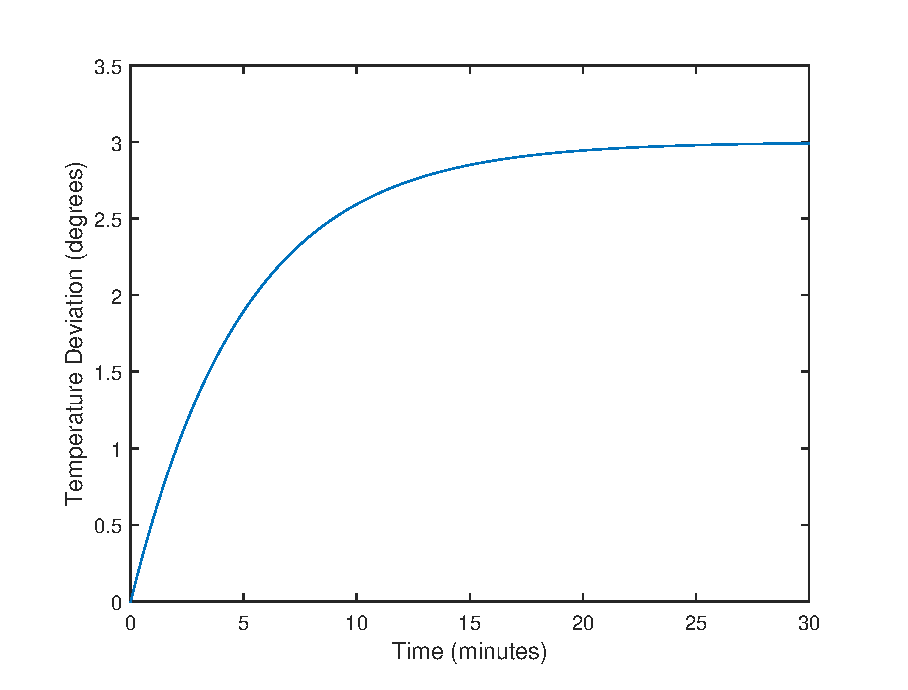
\includegraphics[height=6cm]{1b_mod}
\caption{Temperature deviation model, shown in equation (12), for a step change in the feed temperature of 10$\si{\degreeCelsius}$, holding the heat input constant}
\end{minipage}
\hspace{1cm}
\begin{minipage}{0.45\textwidth}
\centering
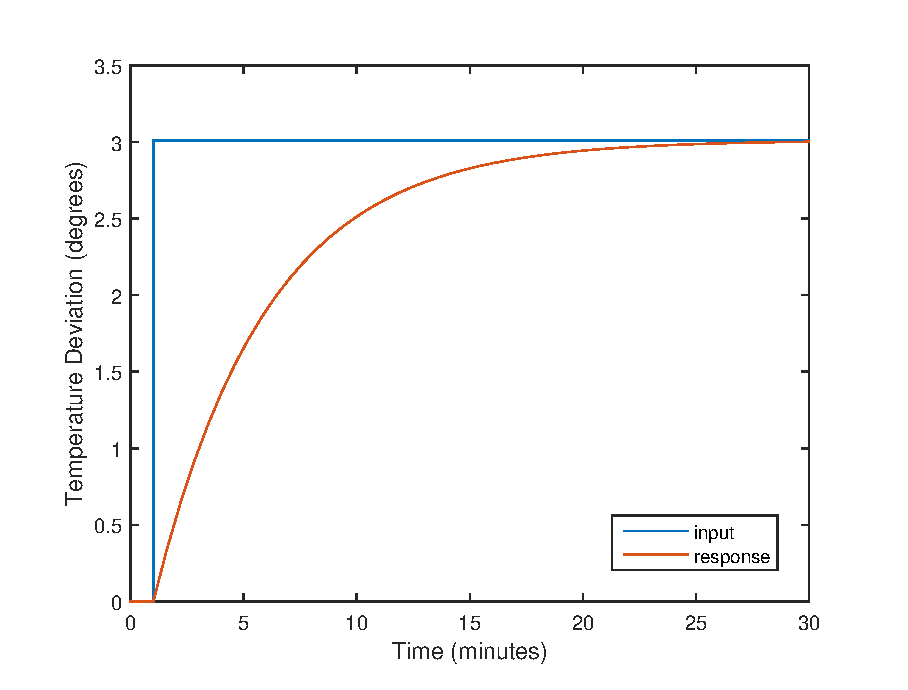
\includegraphics[height=6cm]{1b_sim}
\caption{Temperature deviation simulation for a step change in the feed temperature of 10$\si{\degreeCelsius}$, holding the heat input constant}
\end{minipage}
\end{figure}

\subsection{Time Response for Step Increase in Feed Temperature and Input Heat}

A step increase in the heat input and the feed temperature has a mathematical model in the Laplace domain which is shown in equation (XX):
\begin{align}
T'(s) = \frac{\sfrac{1}{836.8}}{5 \cdot \tau + 1} \cdot q'_h(s)
\end{align} 

Given a deviation in the heat input, $q'_h(t)$ , of 42$\si{\kilo\watt} = 2520\si{\kilo\joule\per\minute}$, we note that the Laplace transform is:
\begin{align*}
\mathscr{L}\{q'_h(t)\} &= \mathscr{L}\{2520 \cdot u(t)\}\\
q'_h(s) &= \frac{2520}{s}
\end{align*}

The mathematical model, in the Laplace domain, becomes:
\begin{align}
T'(s) = \frac{2520}{s \cdot (5 \cdot s + 1)}
\end{align}

Solving this system yields the following expression for the temperature deviation in the time domain:
\begin{align}
T'(t) = 3 \cdot (1 - e^{-\sfrac{t}{5}})
\end{align}

The plot of this model can be seen in Figure XX. A simulation of the system was run in Simulink using the block diagram shown in Figure XX. The step input, and simulated system response can be seen in Figure XX.

\begin{figure}[h]
\centering
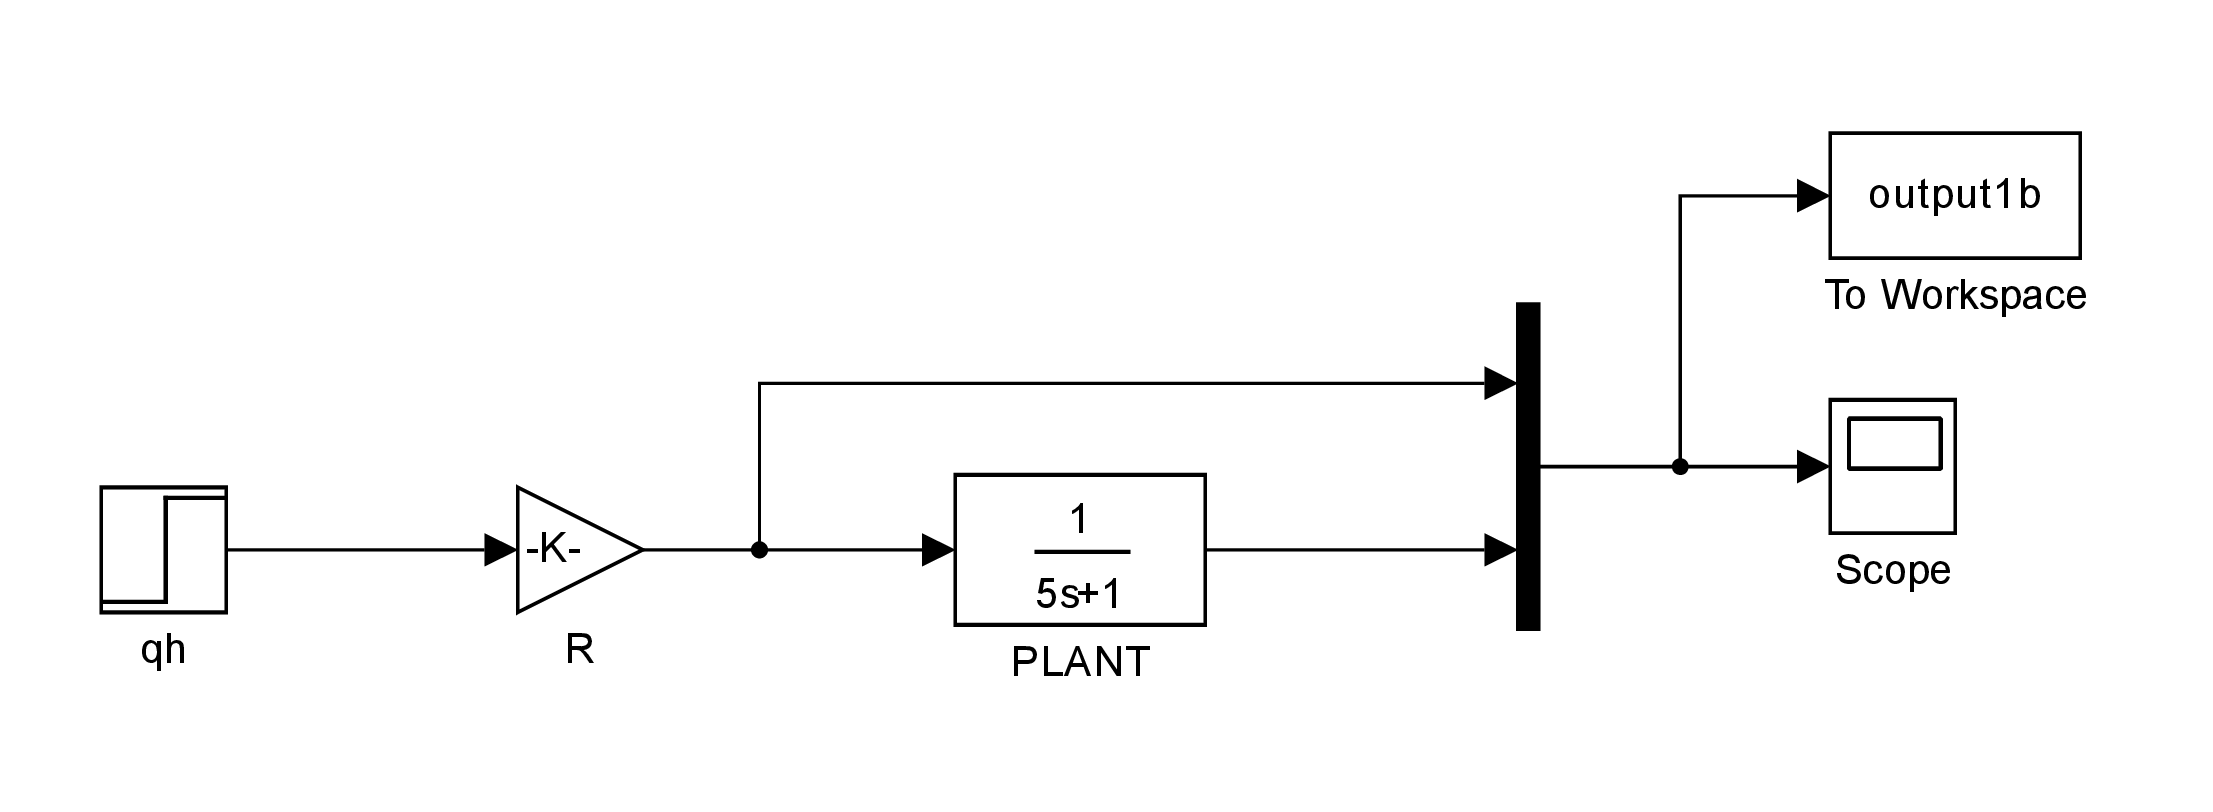
\includegraphics[scale=0.2]{block_1b}
\caption{text}
\end{figure}

\begin{figure}[h]
\begin{minipage}{0.45\textwidth}
\centering
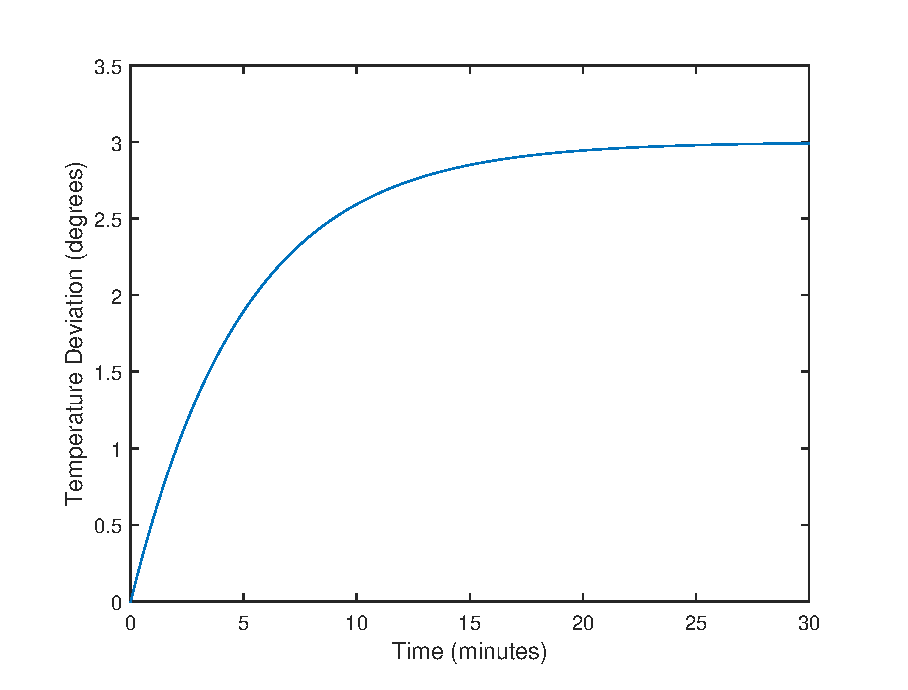
\includegraphics[height=6cm]{1b_mod}
\caption{Temperature deviation model, shown in equation (12), for a step change in the feed temperature of 10$\si{\degreeCelsius}$, holding the heat input constant}
\end{minipage}
\hspace{1cm}
\begin{minipage}{0.45\textwidth}
\centering
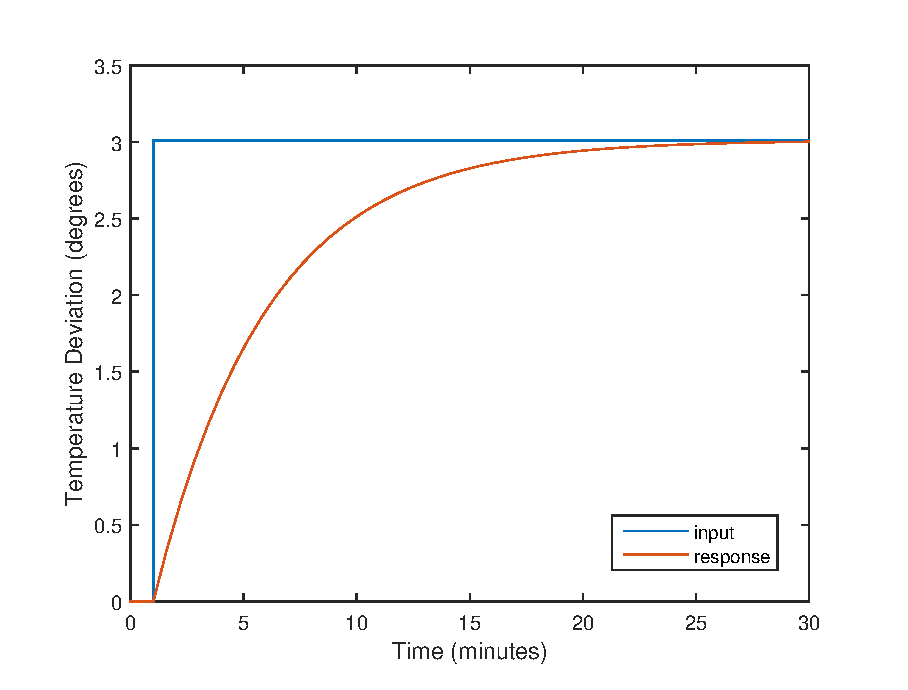
\includegraphics[height=6cm]{1b_sim}
\caption{Temperature deviation simulation for a step change in the feed temperature of 10$\si{\degreeCelsius}$, holding the heat input constant}
\end{minipage}
\end{figure}


%----------------------------------------------------------------------------------------
%	SECTION 3
%----------------------------------------------------------------------------------------

\section{Conclusion}




\end{document}